\section{Backtesting Trading Strategies}
\label{chap:backtesting}

The quantitative evaluation of trading strategies requires a structured and comprehensible testing environment which was introduced in \autoref{chap:te}.
This chapter describes the executed backtests, which aim to verify the performance of the develop trading strategies in \autoref{chap:trading-strategies} under realistic conditions.

Backtesting describes a performance simulation of a trading strategy based on historical data.
This involves investigating how a specific strategy would have performed in the past if it had been executed under the given market conditions.
The goal is to gain initial insights into the robustness, profitability, and risk profile of the approach before it is used in live trading \cite{backtesting}.

\subsection{Trading Strategy Parameter Selection}

In contrast to the classic machine learning process, the parameter selection for the ultimately executed strategies is performed without the training set.
This also applies to strategies that use deep learning (\autoref{chap:ai-strategies}).
Unlike the training of deep learning models, which learn from the training data and adapt their internal states based on the training data, the trading strategies are initialized with fixed parameters.
This corresponds to the fitting of deep learning models.
However, the subsequent process is identical.
The strategies are validated with their previously defined parameters on the validation set to find the best possible parameters.

\subsection{Executing Backtests}

Due to the large number of parameter combinations shown in \autoref{tbl:parameters-number}, backtesting all combinations is not possible due to the execution time.
Therefore, only 1000 combinations per strategy were tested on the validation set.
In order to cover the greatest possible variance of the parameters, the combinations were not sampled randomly from the set of all possible combinations, but the combinations were sorted in lexicographic order and sampled at constant intervals.

\begin{table}[H]
    \centering
    \begin{tabular}{L{8cm}c}
        \toprule
        Strategy Name & Number of Parameters
        \\
        \midrule
        \textbf{Regression AI Strategy}                     & 8,820     \\
        \textbf{Classification AI Strategy}                 & 5,600     \\
        \textbf{Dual Simple Moving Average Strategy}        & 98,000    \\
        \textbf{Triple Exponential Moving Average Strategy} & 1,555,200 \\
        \textbf{Bollinger Bands Strategy}                   & 8,320     \\
        \bottomrule
    \end{tabular}
    \caption{Number of Parameters per Strategy}
    \label{tbl:parameters-number}
\end{table}

\subsection{Evaluating Backtests}

Due to the length, the detailed results of the backtests, including the parameters that led to the respective results, can be found in \autoref{chap:backtest-results} in the appendix.
Here, only the results of the strategies with the highest cumulative last equity combined across all market regimes are presented.

\begin{table}[H]
    \centering
\begin{tabular}{ll|cccc}
    \toprule
    \multicolumn{2}{r|}{Strategy} & \begin{tabular}[c]{@{}c@{}}
                                        Classification\\AI
    \end{tabular} & Dual SMA & Triple EMA & \begin{tabular}[c]{@{}c@{}}
                                                Bollinger\\Bands
    \end{tabular} \\
    \midrule
    \multicolumn{2}{l|}{\textbf{Number of Trades}} & 267 & 3473 & 870 & 275 \\
    \multicolumn{2}{l|}{\textbf{Maximum Gain}} & 956 & 357 & 875 & 191 \\
    \multicolumn{2}{l|}{\textbf{Maximum Loss}} & -245 & -160 & -135 & -64 \\
    \multicolumn{2}{l|}{\textbf{Profits Std.}} & 280 & 37 & 105 & 41 \\
    \multirow{3}{*}{\textbf{Equity}} & \textbf{Minimum} & -2404 & -23   & -75   & 49   \\
    & \textbf{Maximum} & 57908 & 15510 & 10717 & 2510 \\
    & \textbf{Last}    & 55567 & 15159 & 9502  & 2510 \\
    \multicolumn{2}{l|}{\textbf{Maximum Drawdown}} & 4 & 149 & 126 & 51 \\
    \multicolumn{2}{l|}{\textbf{Win Ratio}} & 64 & 49 & 33 & 42 \\
    \bottomrule
\end{tabular}

    \caption{Combined Strategy Results}
    \label{tbl:combined-strategy-results}
\end{table}

As seen in \autoref{tbl:combined-strategy-results} the Classification AI strategy achieves by far the best cumulative results on the validation set, with the lowest maximum drawdown and the highest win ratio.
But on the other hand, it also has the greatest loss.

To compare the out-of-sample performance, all strategies have also been tested with the best parameters on the validation set on the backtest set.

\begin{table}[H]
    \centering
\begin{tabular}{ll|cccc}
    \toprule
    \multicolumn{2}{r|}{Strategy} & \begin{tabular}[c]{@{}c@{}}
                                        Classification\\AI
    \end{tabular} & Dual SMA & Triple EMA & \begin{tabular}[c]{@{}c@{}}
                                                Bollinger\\Bands
    \end{tabular} \\
    \midrule
    \multicolumn{2}{l|}{Number of Trades} & 173 & 5494 & 553 & 444 \\
    \multicolumn{2}{l|}{Maximum Gain} & 424 & 268 & 937 & 163 \\
    \multicolumn{2}{l|}{Maximum Loss} & -144 & -63 & -207 & -88 \\
    \multicolumn{2}{l|}{Profits Std.} & 92 & 9 & 179 & 32 \\
    \multirow{3}{*}{Equity} & Minimum & -2630 & -4694 & -948 & -4378 \\
    & Maximum & 2630  & 0     & 4048 & 0     \\
    & Last    & -2630 & -4694 & 560  & -4365 \\
    \multicolumn{2}{l|}{Maximum Drawdown} & 200 & 898314 & 131 & 87 \\
    \multicolumn{2}{l|}{Win Ratio} & 23 & 26 & 19 & 25 \\
    \bottomrule
\end{tabular}

    \caption{Combined Out-of-Sample Strytegy Results}
    \label{tbl:combined-strategy-results-oof}
\end{table}


\begin{figure}[htbp]
    \centering
    \subfigure[Bild 1]{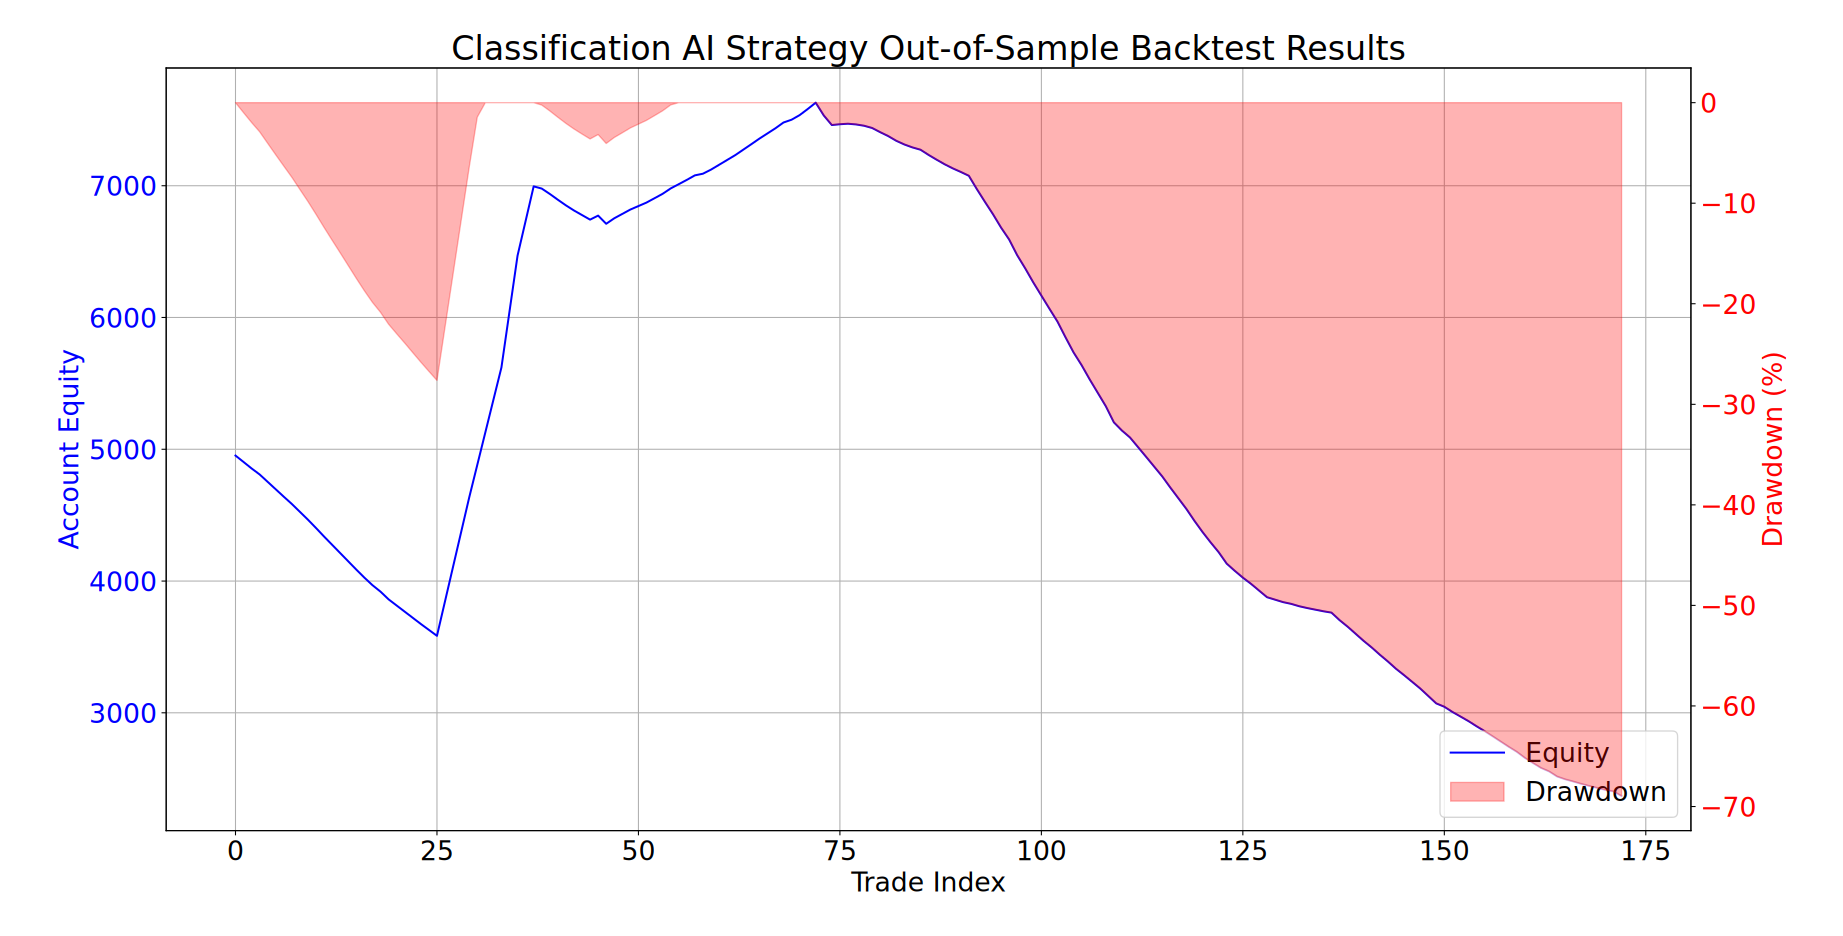
\includegraphics[width=0.45\linewidth]{images/backtests/classification-results-oof}}
    \hfill
    \subfigure[Bild 2]{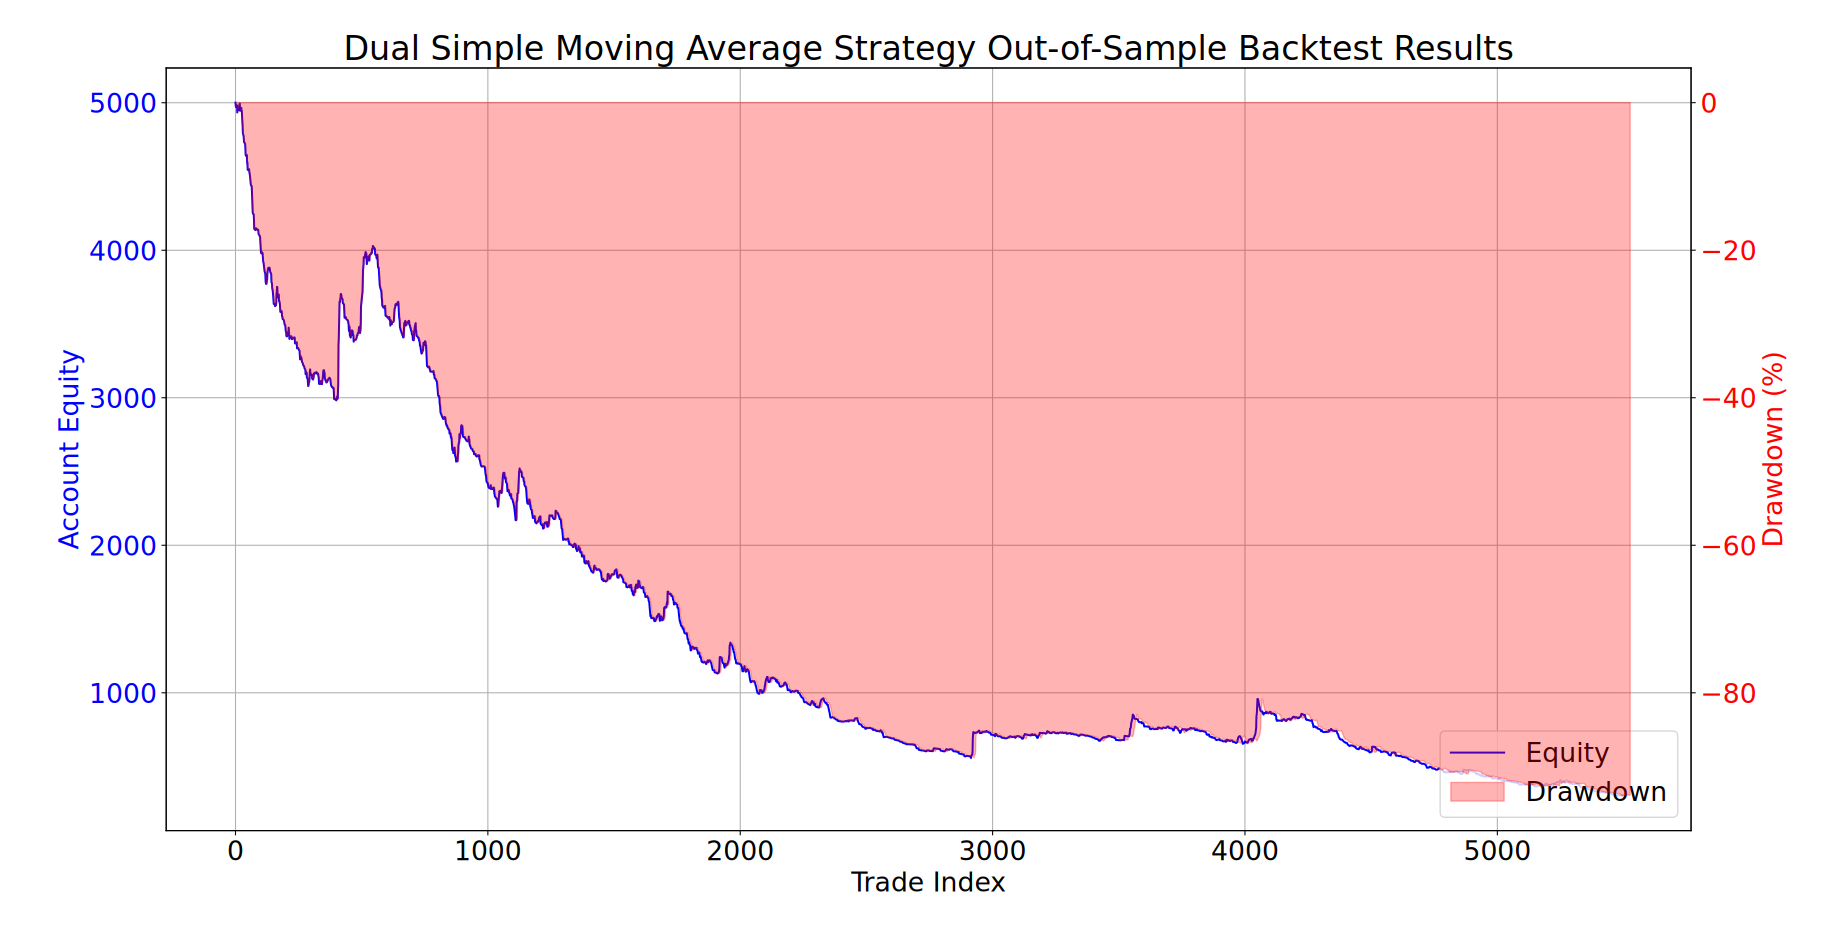
\includegraphics[width=0.45\linewidth]{images/backtests/dual-sma-results-oof}}

    \vspace{0.5cm}

    \subfigure[Bild 3]{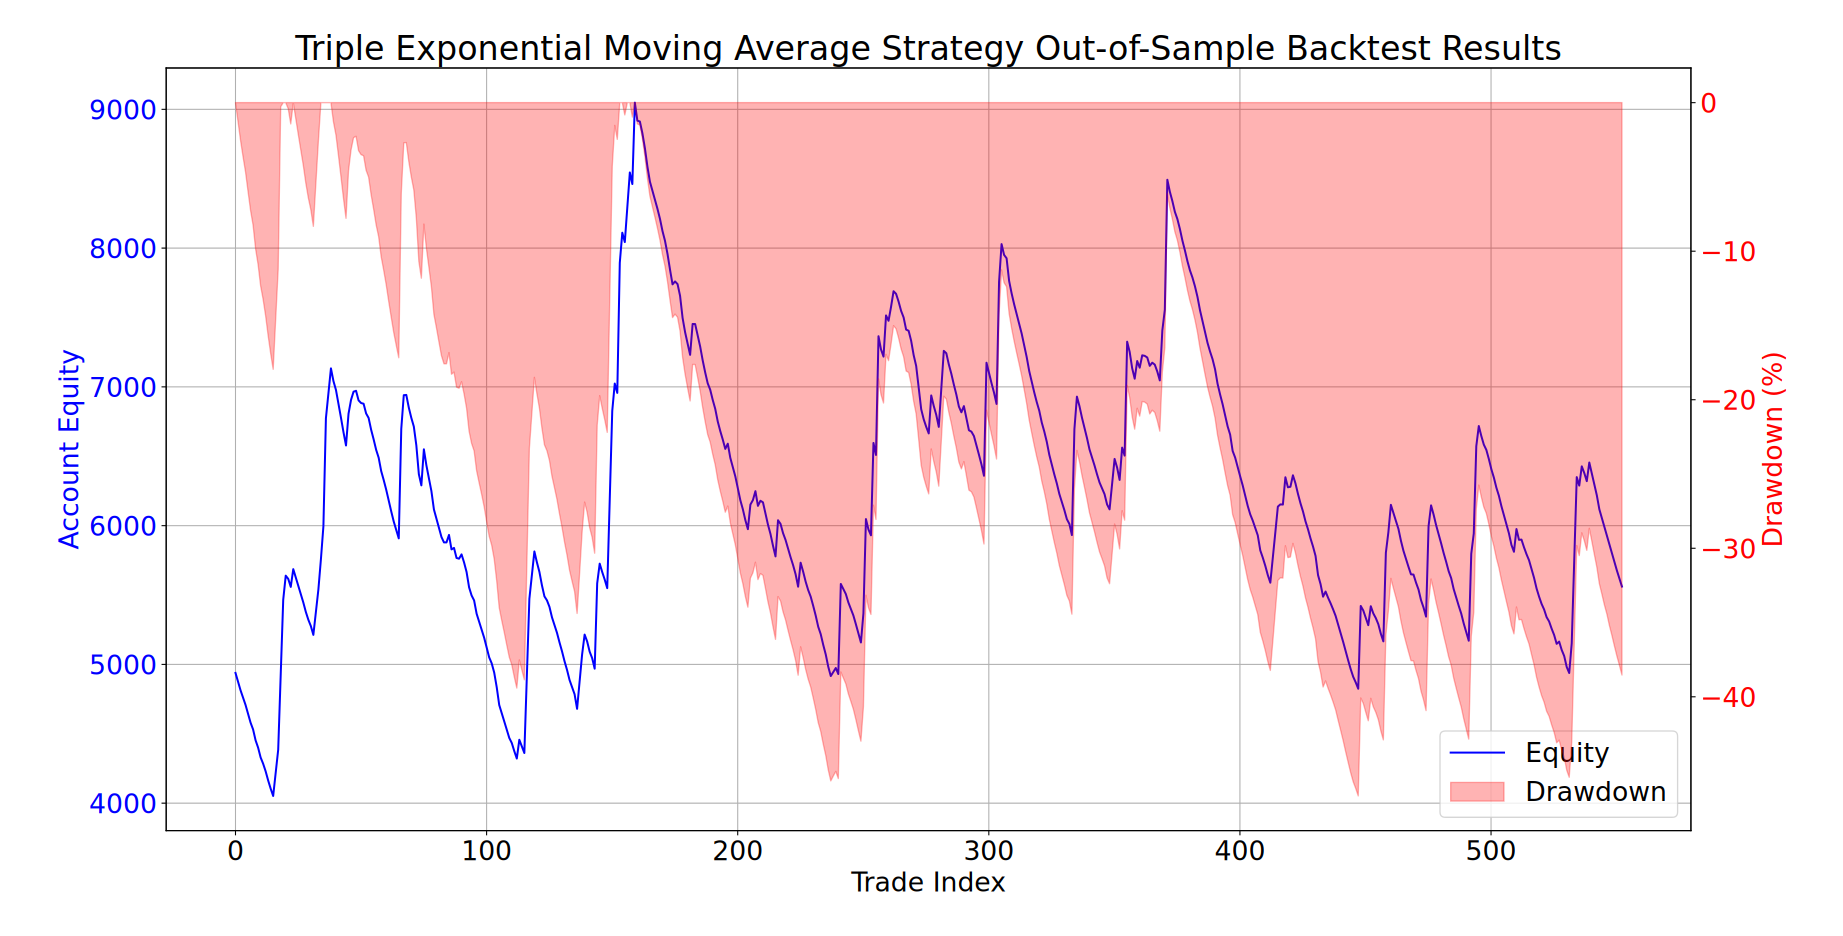
\includegraphics[width=0.45\linewidth]{images/backtests/triple-ema-results-oof}}
    \hfill
    \subfigure[Bild 4]{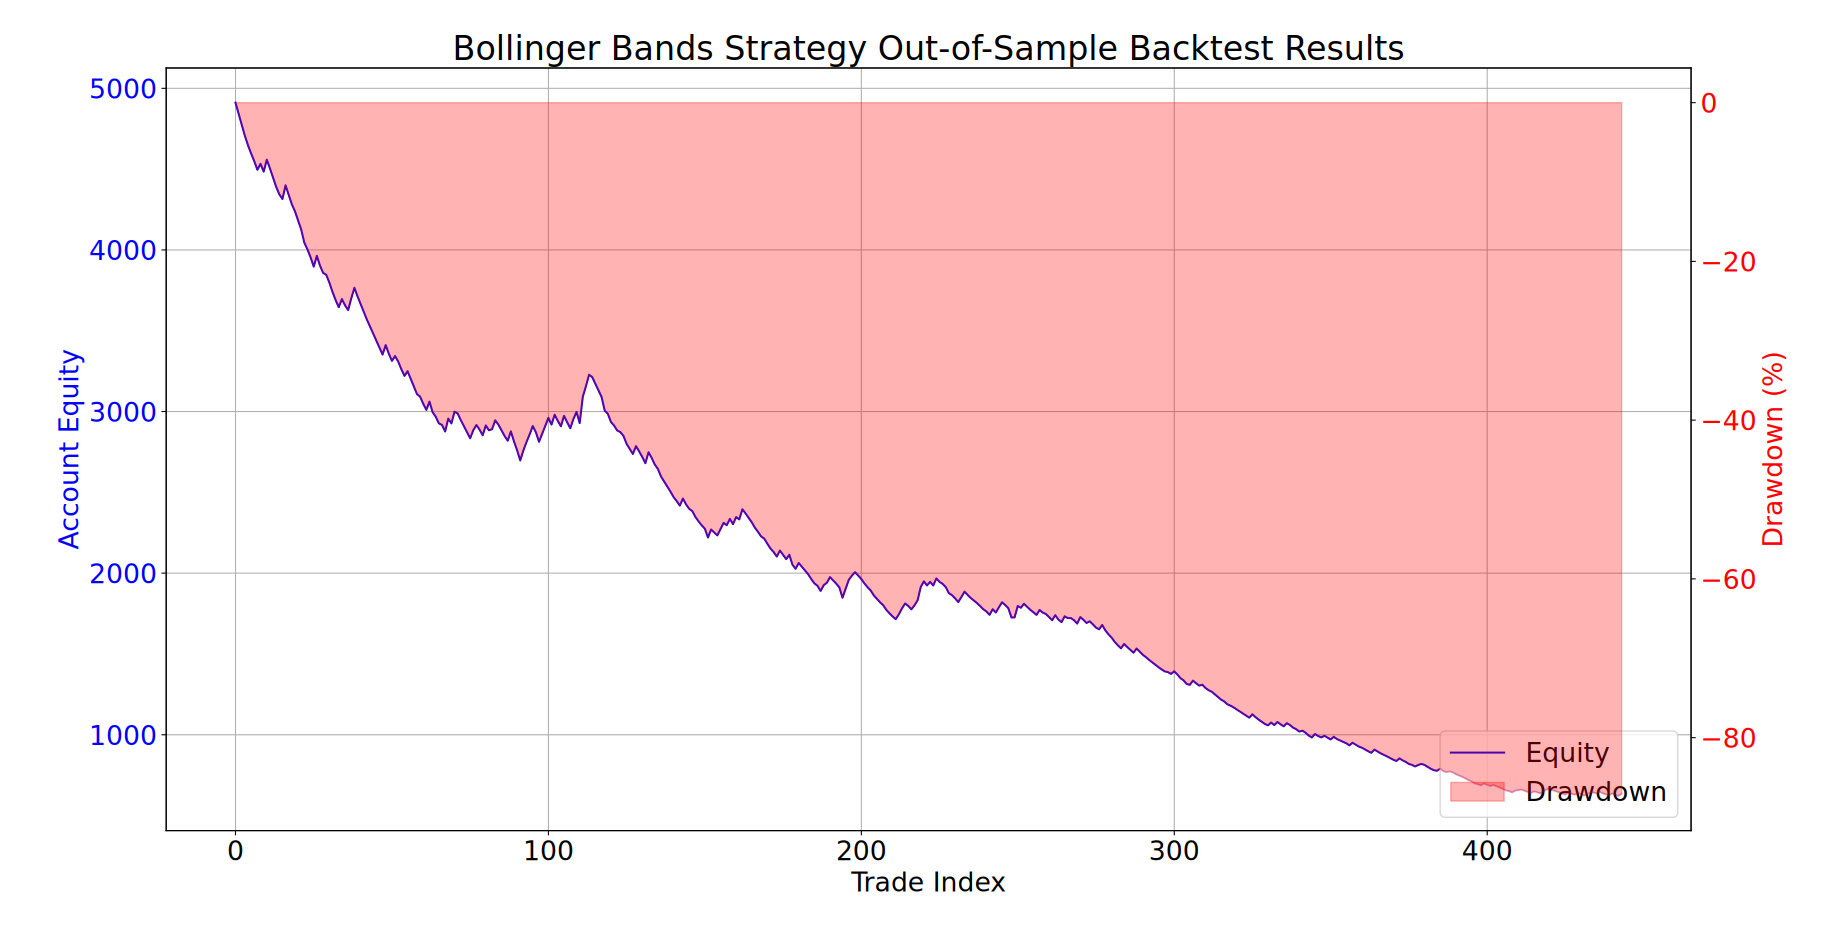
\includegraphics[width=0.45\linewidth]{images/backtests/bb-results-oof}}

    \caption{Vier PDF-Bilder im 2×2-Grid (mit subfigure)}
\end{figure}


\autoref{tbl:combined-strategy-results-oof} shows that the strategies have a poor out-of-sample performance, resulting in either high losses or very volatile equity curves, which are not useful for real live trading.
This shows that there is also a kind of overfitting in the parameter selection.
While the strategies work well on the validation data, they fail in the out-of-sample tests.

\subsection{Fee-Impacts}
